
%% bare_conf.tex
%% V1.4b
%% 2015/08/26
%% by Michael Shell
%% See:
%% http://www.michaelshell.org/
%% for current contact information.
%%
%% This is a skeleton file demonstrating the use of IEEEtran.cls
%% (requires IEEEtran.cls version 1.8b or later) with an IEEE
%% conference paper.
%%
%% Support sites:
%% http://www.michaelshell.org/tex/ieeetran/
%% http://www.ctan.org/pkg/ieeetran
%% and
%% http://www.ieee.org/

%%*************************************************************************
%% Legal Notice:
%% This code is offered as-is without any warranty either expressed or
%% implied; without even the implied warranty of MERCHANTABILITY or
%% FITNESS FOR A PARTICULAR PURPOSE! 
%% User assumes all risk.
%% In no event shall the IEEE or any contributor to this code be liable for
%% any damages or losses, including, but not limited to, incidental,
%% consequential, or any other damages, resulting from the use or misuse
%% of any information contained here.
%%
%% All comments are the opinions of their respective authors and are not
%% necessarily endorsed by the IEEE.
%%
%% This work is distributed under the LaTeX Project Public License (LPPL)
%% ( http://www.latex-project.org/ ) version 1.3, and may be freely used,
%% distributed and modified. A copy of the LPPL, version 1.3, is included
%% in the base LaTeX documentation of all distributions of LaTeX released
%% 2003/12/01 or later.
%% Retain all contribution notices and credits.
%% ** Modified files should be clearly indicated as such, including  **
%% ** renaming them and changing author support contact information. **
%%*************************************************************************


% *** Authors should verify (and, if needed, correct) their LaTeX system  ***
% *** with the testflow diagnostic prior to trusting their LaTeX platform ***
% *** with production work. The IEEE's font choices and paper sizes can   ***
% *** trigger bugs that do not appear when using other class files.       ***                          ***
% The testflow support page is at:
% http://www.michaelshell.org/tex/testflow/



\documentclass[conference]{IEEEtran}


% Some Computer Society conferences also require the compsoc mode option,
% but others use the standard conference format.
%
% If IEEEtran.cls has not been installed into the LaTeX system files,
% manually specify the path to it like:
% \documentclass[conference]{../sty/IEEEtran}





% Some very useful LaTeX packages include:
% (uncomment the ones you want to load)


% *** MISC UTILITY PACKAGES ***
%
%\usepackage{ifpdf}
% Heiko Oberdiek's ifpdf.sty is very useful if you need conditional
% compilation based on whether the output is pdf or dvi.
% usage:
% \ifpdf
%   % pdf code
% \else
%   % dvi code
% \fi
% The latest version of ifpdf.sty can be obtained from:
% http://www.ctan.org/pkg/ifpdf
% Also, note that IEEEtran.cls V1.7 and later provides a builtin
% \ifCLASSINFOpdf conditional that works the same way.
% When switching from latex to pdflatex and vice-versa, the compiler may
% have to be run twice to clear warning/error messages.





\usepackage{mathptmx}
\usepackage[T1]{fontenc}

\usepackage{tabularx}

% Figures
\newcommand\textfig{1cm}
\usepackage{float}
\usepackage{rotating}
\usepackage[tight]{subfigure}
\usepackage{graphicx}

% algo
\usepackage{algorithm}
\usepackage{algorithmicx}
\usepackage{amsmath}
\usepackage{algpseudocode}
\algdef{SE}[DOWHILE]{Do}{DoWhile}{\algorithmicdo}[1]{\algorithmicwhile\ #1}%
\renewcommand{\algorithmicrequire}{\textbf{Input:}}
\renewcommand{\algorithmicensure}{\textbf{Output:}}
\newcommand{\var}[1]{\text{\texttt{#1}}}
\newcommand{\func}[1]{\text{\textsl{#1}}}

% table
\usepackage[normalem]{ulem}
\useunder{\uline}{\ul}{}
\usepackage{multirow}
\usepackage{tabularx}
% *** CITATION PACKAGES ***
%
%\usepackage{cite}
% cite.sty was written by Donald Arseneau
% V1.6 and later of IEEEtran pre-defines the format of the cite.sty package
% \cite{} output to follow that of the IEEE. Loading the cite package will
% result in citation numbers being automatically sorted and properly
% "compressed/ranged". e.g., [1], [9], [2], [7], [5], [6] without using
% cite.sty will become [1], [2], [5]--[7], [9] using cite.sty. cite.sty's
% \cite will automatically add leading space, if needed. Use cite.sty's
% noadjust option (cite.sty V3.8 and later) if you want to turn this off
% such as if a citation ever needs to be enclosed in parenthesis.
% cite.sty is already installed on most LaTeX systems. Be sure and use
% version 5.0 (2009-03-20) and later if using hyperref.sty.
% The latest version can be obtained at:
% http://www.ctan.org/pkg/cite
% The documentation is contained in the cite.sty file itself.






% *** GRAPHICS RELATED PACKAGES ***
%
\ifCLASSINFOpdf
  % \usepackage[pdftex]{graphicx}
  % declare the path(s) where your graphic files are
  % \graphicspath{{../pdf/}{../jpeg/}}
  % and their extensions so you won't have to specify these with
  % every instance of \includegraphics
  % \DeclareGraphicsExtensions{.pdf,.jpeg,.png}
\else
  % or other class option (dvipsone, dvipdf, if not using dvips). graphicx
  % will default to the driver specified in the system graphics.cfg if no
  % driver is specified.
  % \usepackage[dvips]{graphicx}
  % declare the path(s) where your graphic files are
  % \graphicspath{{../eps/}}
  % and their extensions so you won't have to specify these with
  % every instance of \includegraphics
  % \DeclareGraphicsExtensions{.eps}
\fi
% graphicx was written by David Carlisle and Sebastian Rahtz. It is
% required if you want graphics, photos, etc. graphicx.sty is already
% installed on most LaTeX systems. The latest version and documentation
% can be obtained at: 
% http://www.ctan.org/pkg/graphicx
% Another good source of documentation is "Using Imported Graphics in
% LaTeX2e" by Keith Reckdahl which can be found at:
% http://www.ctan.org/pkg/epslatex
%
% latex, and pdflatex in dvi mode, support graphics in encapsulated
% postscript (.eps) format. pdflatex in pdf mode supports graphics
% in .pdf, .jpeg, .png and .mps (metapost) formats. Users should ensure
% that all non-photo figures use a vector format (.eps, .pdf, .mps) and
% not a bitmapped formats (.jpeg, .png). The IEEE frowns on bitmapped formats
% which can result in "jaggedy"/blurry rendering of lines and letters as
% well as large increases in file sizes.
%
% You can find documentation about the pdfTeX application at:
% http://www.tug.org/applications/pdftex





% *** MATH PACKAGES ***
%
%\usepackage{amsmath}
% A popular package from the American Mathematical Society that provides
% many useful and powerful commands for dealing with mathematics.
%
% Note that the amsmath package sets \interdisplaylinepenalty to 10000
% thus preventing page breaks from occurring within multiline equations. Use:
%\interdisplaylinepenalty=2500
% after loading amsmath to restore such page breaks as IEEEtran.cls normally
% does. amsmath.sty is already installed on most LaTeX systems. The latest
% version and documentation can be obtained at:
% http://www.ctan.org/pkg/amsmath





% *** SPECIALIZED LIST PACKAGES ***
%
%\usepackage{algorithmic}
% algorithmic.sty was written by Peter Williams and Rogerio Brito.
% This package provides an algorithmic environment fo describing algorithms.
% You can use the algorithmic environment in-text or within a figure
% environment to provide for a floating algorithm. Do NOT use the algorithm
% floating environment provided by algorithm.sty (by the same authors) or
% algorithm2e.sty (by Christophe Fiorio) as the IEEE does not use dedicated
% algorithm float types and packages that provide these will not provide
% correct IEEE style captions. The latest version and documentation of
% algorithmic.sty can be obtained at:
% http://www.ctan.org/pkg/algorithms
% Also of interest may be the (relatively newer and more customizable)
% algorithmicx.sty package by Szasz Janos:
% http://www.ctan.org/pkg/algorithmicx




% *** ALIGNMENT PACKAGES ***
%
%\usepackage{array}
% Frank Mittelbach's and David Carlisle's array.sty patches and improves
% the standard LaTeX2e array and tabular environments to provide better
% appearance and additional user controls. As the default LaTeX2e table
% generation code is lacking to the point of almost being broken with
% respect to the quality of the end results, all users are strongly
% advised to use an enhanced (at the very least that provided by array.sty)
% set of table tools. array.sty is already installed on most systems. The
% latest version and documentation can be obtained at:
% http://www.ctan.org/pkg/array


% IEEEtran contains the IEEEeqnarray family of commands that can be used to
% generate multiline equations as well as matrices, tables, etc., of high
% quality.




% *** SUBFIGURE PACKAGES ***
%\ifCLASSOPTIONcompsoc
%  \usepackage[caption=false,font=normalsize,labelfont=sf,textfont=sf]{subfig}
%\else
%  \usepackage[caption=false,font=footnotesize]{subfig}
%\fi
% subfig.sty, written by Steven Douglas Cochran, is the modern replacement
% for subfigure.sty, the latter of which is no longer maintained and is
% incompatible with some LaTeX packages including fixltx2e. However,
% subfig.sty requires and automatically loads Axel Sommerfeldt's caption.sty
% which will override IEEEtran.cls' handling of captions and this will result
% in non-IEEE style figure/table captions. To prevent this problem, be sure
% and invoke subfig.sty's "caption=false" package option (available since
% subfig.sty version 1.3, 2005/06/28) as this is will preserve IEEEtran.cls
% handling of captions.
% Note that the Computer Society format requires a larger sans serif font
% than the serif footnote size font used in traditional IEEE formatting
% and thus the need to invoke different subfig.sty package options depending
% on whether compsoc mode has been enabled.
%
% The latest version and documentation of subfig.sty can be obtained at:
% http://www.ctan.org/pkg/subfig




% *** FLOAT PACKAGES ***
%
%\usepackage{fixltx2e}
% fixltx2e, the successor to the earlier fix2col.sty, was written by
% Frank Mittelbach and David Carlisle. This package corrects a few problems
% in the LaTeX2e kernel, the most notable of which is that in current
% LaTeX2e releases, the ordering of single and double column floats is not
% guaranteed to be preserved. Thus, an unpatched LaTeX2e can allow a
% single column figure to be placed prior to an earlier double column
% figure.
% Be aware that LaTeX2e kernels dated 2015 and later have fixltx2e.sty's
% corrections already built into the system in which case a warning will
% be issued if an attempt is made to load fixltx2e.sty as it is no longer
% needed.
% The latest version and documentation can be found at:
% http://www.ctan.org/pkg/fixltx2e


%\usepackage{stfloats}
% stfloats.sty was written by Sigitas Tolusis. This package gives LaTeX2e
% the ability to do double column floats at the bottom of the page as well
% as the top. (e.g., "\begin{figure*}[!b]" is not normally possible in
% LaTeX2e). It also provides a command:
%\fnbelowfloat
% to enable the placement of footnotes below bottom floats (the standard
% LaTeX2e kernel puts them above bottom floats). This is an invasive package
% which rewrites many portions of the LaTeX2e float routines. It may not work
% with other packages that modify the LaTeX2e float routines. The latest
% version and documentation can be obtained at:
% http://www.ctan.org/pkg/stfloats
% Do not use the stfloats baselinefloat ability as the IEEE does not allow
% \baselineskip to stretch. Authors submitting work to the IEEE should note
% that the IEEE rarely uses double column equations and that authors should try
% to avoid such use. Do not be tempted to use the cuted.sty or midfloat.sty
% packages (also by Sigitas Tolusis) as the IEEE does not format its papers in
% such ways.
% Do not attempt to use stfloats with fixltx2e as they are incompatible.
% Instead, use Morten Hogholm'a dblfloatfix which combines the features
% of both fixltx2e and stfloats:
%
% \usepackage{dblfloatfix}
% The latest version can be found at:
% http://www.ctan.org/pkg/dblfloatfix




% *** PDF, URL AND HYPERLINK PACKAGES ***
%
\usepackage{url}
% url.sty was written by Donald Arseneau. It provides better support for
% handling and breaking URLs. url.sty is already installed on most LaTeX
% systems. The latest version and documentation can be obtained at:
% http://www.ctan.org/pkg/url
% Basically, \url{my_url_here}.




% *** Do not adjust lengths that control margins, column widths, etc. ***
% *** Do not use packages that alter fonts (such as pslatex).         ***
% There should be no need to do such things with IEEEtran.cls V1.6 and later.
% (Unless specifically asked to do so by the journal or conference you plan
% to submit to, of course. )


% correct bad hyphenation here
\hyphenation{op-tical net-works semi-conduc-tor}


\begin{document}
%
% paper title
% Titles are generally capitalized except for words such as a, an, and, as,
% at, but, by, for, in, nor, of, on, or, the, to and up, which are usually
% not capitalized unless they are the first or last word of the title.
% Linebreaks \\ can be used within to get better formatting as desired.
% Do not put math or special symbols in the title.
\title{DeAr: A Framework for Power-efficient and Flexible Embedded Digital Signal Processor Design}


% author names and affiliations
% use a multiple column layout for up to three different
% affiliations
\author{\IEEEauthorblockN{Chi-Ming~Lee\IEEEauthorrefmark{1}, Shih-Hao~Ou\IEEEauthorrefmark{4}, Chih-Wei~Liu\IEEEauthorrefmark{3} ,Yarsun~Hsu\IEEEauthorrefmark{2} }
    \IEEEauthorblockA{\IEEEauthorrefmark{1}\IEEEauthorrefmark{2}Department of Electrical Engineering, National Tsing Hua University, Taiwan}
    \IEEEauthorblockA{\IEEEauthorrefmark{3}\IEEEauthorrefmark{4}Department of Electronics Engineering, National Chiao Tung University, Taiwan}
    \IEEEauthorblockA{Email: \IEEEauthorrefmark{1}cm99585@hotmail.com, \IEEEauthorrefmark{4}shou@twins.ee.nctu.edu.tw, \IEEEauthorrefmark{3}cwliu@twins.ee.nctu.edu.tw, \IEEEauthorrefmark{2}yshsu@ee.nthu.edu.tw }
}

% conference papers do not typically use \thanks and this command
% is locked out in conference mode. If really needed, such as for
% the acknowledgment of grants, issue a \IEEEoverridecommandlockouts
% after \documentclass

% for over three affiliations, or if they all won't fit within the width
% of the page, use this alternative format:
% 
%\author{\IEEEauthorblockN{Michael Shell\IEEEauthorrefmark{1},
%Homer Simpson\IEEEauthorrefmark{2},
%James Kirk\IEEEauthorrefmark{3}, 
%Montgomery Scott\IEEEauthorrefmark{3} and
%Eldon Tyrell\IEEEauthorrefmark{4}}
%\IEEEauthorblockA{\IEEEauthorrefmark{1}School of Electrical and Computer Engineering\\
%Georgia Institute of Technology,
%Atlanta, Georgia 30332--0250\\ Email: see http://www.michaelshell.org/contact.html}
%\IEEEauthorblockA{\IEEEauthorrefmark{2}Twentieth Century Fox, Springfield, USA\\
%Email: homer@thesimpsons.com}
%\IEEEauthorblockA{\IEEEauthorrefmark{3}Starfleet Academy, San Francisco, California 96678-2391\\
%Telephone: (800) 555--1212, Fax: (888) 555--1212}
%\IEEEauthorblockA{\IEEEauthorrefmark{4}Tyrell Inc., 123 Replicant Street, Los Angeles, California 90210--4321}}




% use for special paper notices
%\IEEEspecialpapernotice{(Invited Paper)}




% make the title area
\maketitle

% As a general rule, do not put math, special symbols or citations
% in the abstract
\begin{abstract}
    The evolution of wireless communication protocols drives the quest of power-efficient and flexible computing for embedded DSPs, 
    but popular architectures, very-long-instruction-word (VLIW) and application-specific instruction set processor (ASIP), serve as opposite extreme cases in regard to power-efficiency and flexibility.
    To this end, we present DeAr: Dual-thread Architecture DSP, 
    which manipulates a multi-banked register file that enables simultaneous multi-threading (SMT),
    and a transport-triggered bus that exploits the data forwarding mechanism in its compact datapath.
    We also propose a novel scheduling algorithm which leverages the compact hardware to achieve both high throughput and flexible computation.
    In the experiment of common DSP kernels, 
    DeAr saves 20.3\%--13.1\% and 31.8\%--2.2\% of power dissipation, 36.1\%--31.5\% and 28.2\%--5.7\% of area, compared with VLIW and ASIP respectively.
\end{abstract}

% no keywords




% For peer review papers, you can put extra information on the cover
% page as needed:
% \ifCLASSOPTIONpeerreview
% \begin{center} \bfseries EDICS Category: 3-BBND \end{center}
% \fi
%
% For peerreview papers, this IEEEtran command inserts a page break and
% creates the second title. It will be ignored for other modes.
\IEEEpeerreviewmaketitle

%\section{Introduction}%
As wireless communication standards evolve, the demand for a digital signal processor (DSP) supplying computation with high performance, high flexibility and low power-dissipation is gaining momentum in the mobile industry. 
For example, LTE-advance demands 10 times higher transmission throughput than that of LTE~\cite{lte}, 
and algorithms of LTE-advance could change frequently with protocol specifications.
%To achieve such enhancement, strategies such as scaling up MIMO system and permitting carrier aggregation~\cite{carrier} that require more sophisticated arithmetics are adopted in LTE-advance.
%Consequently, both energy efficiency and flexibility become crucial considerations in the filed of digital signal processor design. 
However, Very Long Instruction Word (VLIW) and Application-Specific Instruction set Processor (ASIP), which have been popular architectures for state-of-the-art DSPs, are considered to be opposite extreme cases by hardware designers who would like to trade-off between flexibility and power-efficiency. 
VLIW gains good flexibility by allocating each arithmetic unit dedicated control signals and data ports in the register file (RF), which result in severe power dissipation. %so it could work orthogonally with each other.
On the contrary, ASIP buys the optimized datapath for a specific ISA or algorithm at the expense of flexibility, so good power-efficiency can be achieved. 
Consequently, improving the power efficiency while keeping the flexibility of a DSP for mobile devices consequently has been a challenge.	
\\\indent
To address this issue, 
we present DeAr, Dual-thread Architecture DSP, with features summarized below: 
\textbf{(1)} The multi-issue datapath enables Simultaneous Multi-threading (SMT).
\textbf{(2)} The transport triggered data bus exhaustively forwards data from accumulator latches to ALU.
\textbf{(3)} Banked organization of the RF eliminates redundant connections from ports to registers.
\textbf{(4)} RF access is simplified to implicit operations (i.e. push or pop) instead of conventional random access.
\\\indent
Besides, we propose a novel program analysis approach based on the hierarchical data flow graph (HDFG), which is an enhanced data flow graph.
With HDFG-based scheduling, DeAr achieves both high throughput and flexibility, 
and exploits data forwarding opportunities to reduce power dissipation.



\section{Introduction}%
As wireless communication standards evolve, the demand for a digital signal processor (DSP) supplying computation with high performance, high flexibility and low power-dissipation is gaining momentum in the mobile industry. 
For example, LTE-advance demands 10 times higher transmission throughput than that of LTE~\cite{lte}, 
and algorithms of LTE-advance could change frequently with protocol specifications.
%To achieve such enhancement, strategies such as scaling up MIMO system and permitting carrier aggregation~\cite{carrier} that require more sophisticated arithmetics are adopted in LTE-advance.
%Consequently, both energy efficiency and flexibility become crucial considerations in the filed of digital signal processor design. 
However, Very Long Instruction Word (VLIW) and Application-Specific Instruction set Processor (ASIP), which have been popular architectures for state-of-the-art DSPs, are considered to be opposite extreme cases by hardware designers who would like to trade-off between flexibility and power-efficiency. 
VLIW gains good flexibility by allocating each arithmetic unit dedicated control signals and data ports in the register file (RF), which result in severe power dissipation. %so it could work orthogonally with each other.
On the contrary, ASIP buys the optimized datapath for a specific ISA or algorithm at the expense of flexibility, so good power-efficiency can be achieved. 
Consequently, improving the power efficiency while keeping the flexibility of a DSP for mobile devices consequently has been a challenge.	
\\\indent
To address this issue, 
we present DeAr, Dual-thread Architecture DSP, with features summarized below: 
\textbf{(1)} The multi-issue datapath enables Simultaneous Multi-threading (SMT).
\textbf{(2)} The transport triggered data bus exhaustively forwards data from accumulator latches to ALU.
\textbf{(3)} Banked organization of the RF eliminates redundant connections from ports to registers.
\textbf{(4)} RF access is simplified to implicit operations (i.e. push or pop) instead of conventional random access.
\\\indent
Besides, we propose a novel program analysis approach based on the hierarchical data flow graph (HDFG), which is an enhanced data flow graph.
With HDFG-based scheduling, DeAr achieves both high throughput and flexibility, 
and exploits data forwarding opportunities to reduce power dissipation.


\section{Related Work}
\label{cha:related}
    Many studies have been conducted on RF organization as it becomes the dominating cost in DSPs\cite{register}.
    %Rixner \textit{et al.} indicated that, for conventional centralized organization of RF, the cost grows significantly with the number of functional units (FUs) \cite{register}, posing a serious challenge to VLIW DSP design.
    A straightforward solution to it is partitioning the centralized RF into several parts, each of which serves specific FUs, such as \cite{cluster}.
    Studies like \cite{synzen} and \cite{dsplite} went even further by discarding the centralized RF and allocating each FU a dedicated one, which is also known as distributed RF organization.
    However, dividing RF leads to more complicated compiler design and overhead of inter-RF data transport.
    In addition, above approaches still suffer from poor code density, which is an inherent problem from the VLIW architecture.
    %\\\indent
    On the other hand, some approaches avoided the aforementioned cost growth by customizing the datapath and reducing the number of ports on RF.
    Ou \textit{et al.} proposed composite FUs for DSP, which cascade FUs with a specific order and demand fewer ports on RF \cite{cascade} \cite{hearaid}.
    Similar techniques are often applied to ASIP design but they usually lack flexibility for general purposes.
    %There are further researches that achieve power reduction on RF by minimizing the number of accesses to it.
    %Chen \textit{et al.} proposed a simulated-annealing based scheduling that aggressively forwards data from FU outputs to inputs instead of accessing RF \cite{multistage}.
    %\cite{move} presented a processor framework: MOVE, which features the separation of data transport and operation in the datapath. 
    %The user can program the bypass network in MOVE, and avoid most of accesses to RF by clever data transport.
    %Such an architecture that manipulates data transport is usually referred to as transport-triggered architecture (TTA).
    %The Work from Lama \textit{et al.} \cite{ttagpu} also demonstrated a framework that takes the advantage of TTA in graphic processing unit (GPU), and this idea is a potential alternative for DSP design.
    %\\\indent
    %On the other hand, one may notices that none of the above implementations adopts HSA \cite{systemspec}, which is a promising standard for embedded DSP platforms.
    %So far, most of studies of HSA focus on the integration of CPU and GPU. 
    %\cite{hsaemu} presented a full system emulator for HSA platforms that include CPUs and GPUs.
    %Beyond emulation, the study on a cycle-accurate HSA simulator that integrates QEMU \cite{qemu} and GPGPU-sim \cite{gpgpusim} is going in full swing.
    %To the best of our knowledge, little or no research has been conducted on applying the standard to DSP platforms.
    %\\\indent
    %Nevertheless, we found that some of studies which aimed at accelerating GPU can be applicable to HSA with DSPs.
    %Hsu \textit{et.al.} proposed a hardware-based memory layout controller for heterogeneous systems~\cite{sc}.
    %The controller optimizes irregular data structures from CPU and fit them to the memory footprint of GPU on-the-flight of memory transfer.
    %The data locality in GPU is improved significantly as well as the latency of data layout conversion is hidden.
    %Such a data conversion mechanism is also crucial to the integration of DeAr DSP and HSA, 
    %and it will be presented with reference to \cite{sc} in Section~\ref{sec:integration}.


%\section{Background}
    \subsection{Evolution of Digital Signal Processors}
        A digital signal processor (DSP) is an optimized computer that aims at accelerating digital signal processing, such as baseband demodulation or video codec.
        In principle, a programmer extracts key subroutines or algorithms from applications and accelerates them with a DSP.
        Such extracted pieces of code that executed by DSPs are also referred to DSP kernels.
        Unlike general purpose computers, which usually feature powerful ISA and novel branch predictors that help them dealing with control intensive tasks very well,
        DSPs simply focus on computation intensive tasks delivered by another unit (general purpose processor, analog to digital converter, etc.), 
        and thus its hardware can be simplified and optimized for better power efficiency, which enable them to be widely used in mobile devices and embedded systems.
        \\\indent
        The single-issue reduced instruction set computer (scalar), introduced in 1980s \cite{risc}, has become a popular template for DSP owing to its simplicity.
        The key concept of scalar is designing an ISA with primitive and orthogonal instructions which demand simpler datapath.
        By taking the advantage of the regularity in its datapath, pipelining technique can thus be adopt to achieve the application requirement.
        However, two drawbacks still exist in scalar. 
        The first its lack of instruction-level parallelism (ILP). 
        Functional units are not able to work concurrently due to the limitation of the single-issue datapath.
        This can be resolved by designing a multi-issue datapath with either hardware (i.e., superscalar) or software (i.e., VLIW) instruction scheduling.
        In the field of DSP design, adopting the VLIW architecture is a preferable strategy, 
        because hardware simplicity matters than portability and many optimization approaches can be applied in compilation stages. 
        Figure~\ref{fig:vliw} illustrates a 3-way issue VLIW datapath, where three instructions can be dispatched at a cycle.
        The number of ports on RF is scaled up with the issue-width, and the compiler is responsible for performing static scheduling to avoid resources conflict among operations.
        \vspace{\textfig}
        \begin{figure}[!ht] 
            \centering
            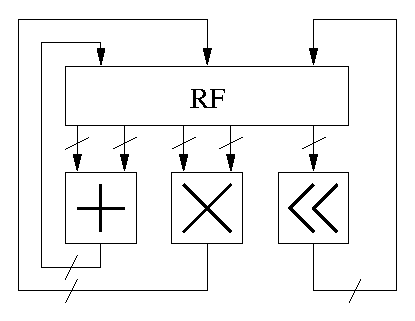
\includegraphics[width=0.5\textwidth]{./figs/vliw.eps}
            \caption{Basic VLIW datapah}
            \label{fig:vliw}
        \end{figure}
        \\\indent
        The second drawback of scalar is plenty of redundant writing back (WB) to RF. 
        In digital signal processing, intermediate results are often read exactly once, which implies lots of RF storage of them is redundant.
        Several approaches have been proposed to address this issue.
        Figure~\ref{fig:cascade} shows the datapath of the composite-ALU architecture that cascades primitive arithmetic units. 
        Intermediate results can be forwarded from one to its follower with an optimized order which targets specific applications.
        The processor with such customization in the datapath is referred to as application-specific instruction set processor (ASIP).
        \vspace{\textfig}
        \begin{figure}[!ht] 
            \centering
            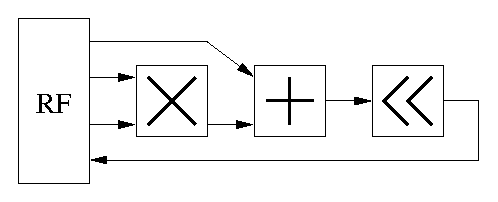
\includegraphics[width=0.6\textwidth]{./figs/cascade.eps}
            \caption{Composite-ALU architecture}
            \label{fig:cascade}
        \end{figure}
        \\\indent
        Another approach that enables forwarding mechanism even further is shown in Figure~\ref{fig:tta}, where FUs, RF and load/store units are linked by an interconnection network (ICN).
        Such an architecture makes a significant distinction from scalar because only a "move" instruction is needed. 
        All computation can be completed by moving operands on the interconnection network, avoiding WB as much as possible.
        \vspace{\textfig}
        \begin{figure}[!ht] 
            \centering
            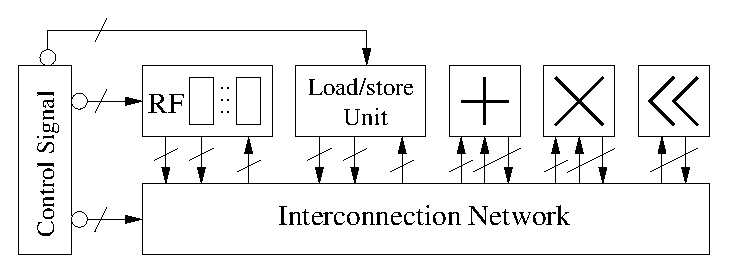
\includegraphics[width=0.8\textwidth]{./figs/tta.eps}
            \caption{Transport triggered architecture (TTA)}
            \label{fig:tta}
        \end{figure}
      
        %\subsubsection{Application-Specific Instruction Set Processor}
        %\subsubsection{Very Long Instruction Word Processor}
        %\subsubsection{Transport-Triggered Architecture}

    %\subsection{Register File Model}
    %Register file (RF) organization also serves as an important role in DSP design. 
    %Increaing computational demand drives more and more FUs on RF,
    %which result in significant hardware cost.
    %In this part, we will introduce a basic RF model to explain hardware cost in area, delay and power perspectives.
    %\subsubsection{Area}
    %\label{sec:area}
    %RF is an array of register cells, each of which connects to several bit lines and word lines.
    %Figure~\ref{fig:rf} illustrates a basic schematic of a register cell.
    %    \vspace{\textfig}
    %    \begin{figure}[!ht] 
    %        \centering
    %        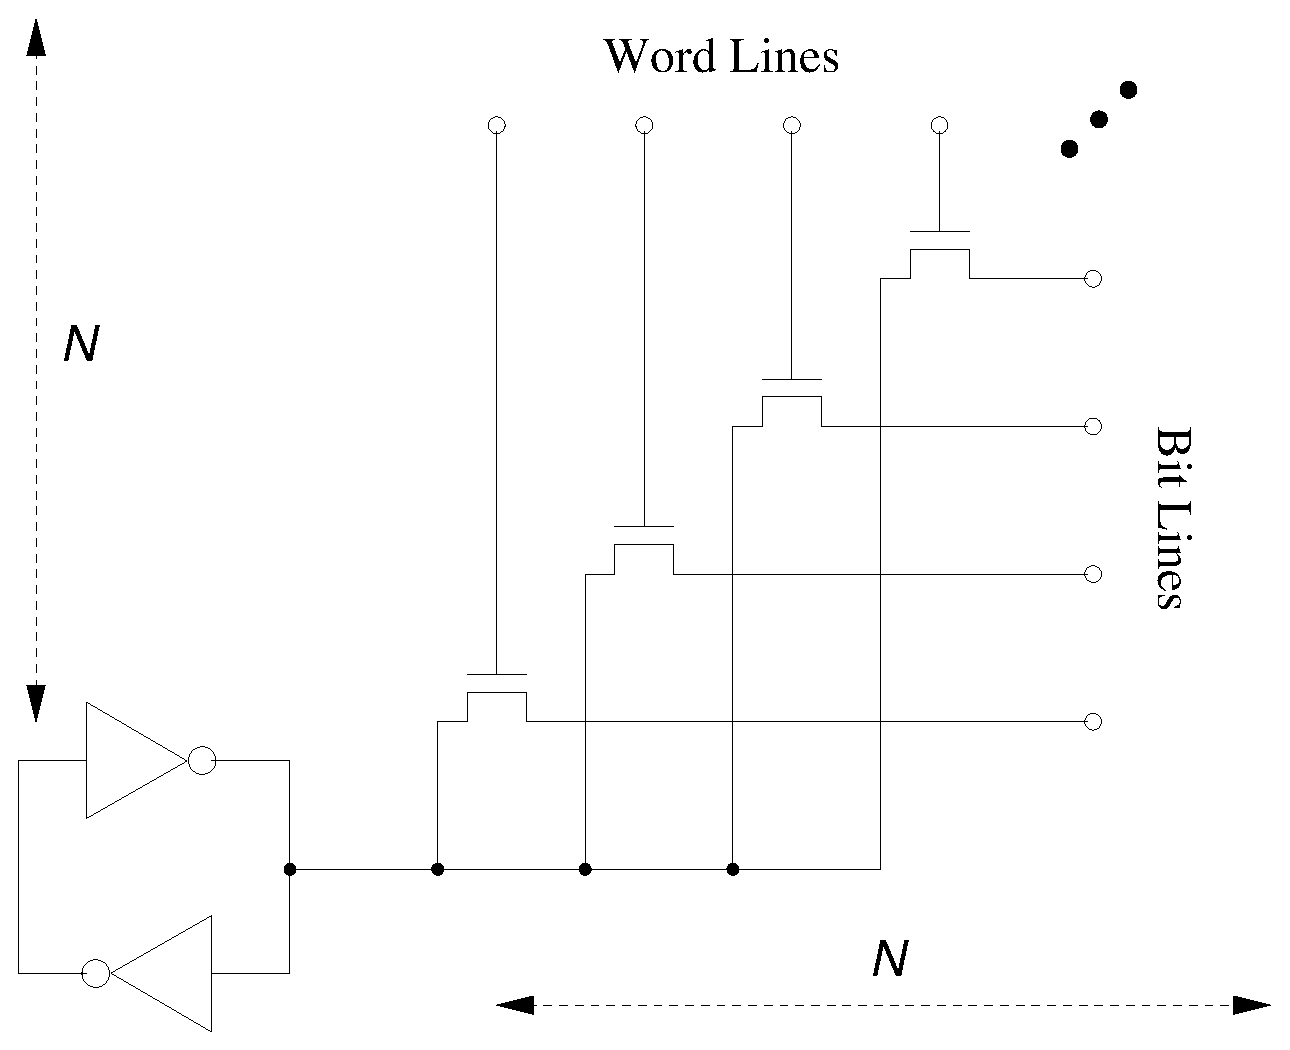
\includegraphics[width=0.7\textwidth]{./figs/rf.eps}
    %        \caption{Register cell schematic}
    %        \label{fig:rf}
    %    \end{figure}
    %For a centralized RF organization with N ports, 
    %each register cell is connected to N bit lines, each of which controlled by a word lines.
    %N bit lines and N word lines are placed horizontally and vertically respectively.
    %Since the width of wire tracks is a constant, 
    %the interconnection area of each cell grows with the factor of $N^2$.
    %Moreover, since the register number grows with the FU number as well,
    %the factor of total interconnection area is further multiplied with another N and reaches $N^3$,  
    %which dominates the chip area when N is large.
    %\subsubsection{Delay}
    %Wire propagation and fan-out/fan-in delays are two major constituents of RF access delay.
    %The former is the latency of a logic passage across a wire,
    %which is proportional to the wire length, 
    %while the latter is the latency of driving on capacitive loads.
    %As discussed in ~\ref{sec:area}, the interconnection area of RF is the factor of $N^3$.
    %By taking square root on the factor of area, 
    %we obtain another factor, $N^{3/2}$, for wire length and propagation delay.
    %The growing wire length increases load capacitance on bit lines as well, 
    %and it contribute additional fan-out/fan-in delay to the overall.
    %Nevertheless, $N^{3/2}$ is still the dominating factor of RF access delay when N is large.
    %\subsubsection{Power}
    %For each access to RF, bit lines need to be pre-charged to a threshold voltage,
    %and then sense register cells by asserting specific word lines.
    %As a result, the energy dissipation in RF is mainly resulted from logic switching in bit lines capacitance,
    %because every bit line dedicated to a port needs to be active to accomplish an access to the port.
    %As the port number increases, the capacitance in bit line is principally wire capacitance.
    %The overall power consumption of bit lines grows with the product of the bit line number and the wire length.
    %As shown in Figure~\ref{fig:rf}, the wire length and the bit line number of each cell are proportional to N.
    %Since the register cell number is proportional to N as well, 
    %the overall power consumption of bit lines is also the factor of $N^3$ when N is large.
    %    %\subsubsection{Centralized Register Files}
        %\subsubsection{Banked Register Files}
        %\subsubsection{Clustered Register Files}
        %\subsubsection{Distributed Register Files}
    \subsection{Heterogeneous System Architecture}
    \textit{Heterogeneous System Architecture} (HSA) presents an unified view of various computing devices, 
    such as CPU, DSP, GPU and FPGA.
    HSA allows these devices to be integrated in a single system heterogeneously, and even share the same memory virtually or physically.
    Such asymmetry of computing devices in HSA is the key differentiation from conventional symmetric multiprocessing (SMP) \cite{parallel},
    which involves two or more identical processors collaborating with uniform access to the shared memory.
    By adopting HSA, one is able to design a single system that handles wide variety of computational demands efficiently.
    For example, in 2014, AMD released its fourth generation of the Accelerated Processing Unit (APU), \textit{Carrizo APU} \cite{carrizo}, featuring HSA 1.0.
    As illustrated in Figure~\ref{fig:carrizo}, \textit{Carrizo} is the SoC platform with the 4-core CPU and the GPU with 8 compute units (384 shader cores totally).
    Both of them work with textit{the Shared Virtual Memory} (SVM) since their MMUs access an identical page table.
    \textit{Carrizo} enables task sharing without data copy between CPUs and GPUs to achieve greater performance.
    By cleverly choosing the suitable computing device for each task, 
    \textit{Carrizo} can operate more efficiently to save power as well.
    Since the proposed DeAr DSP targets HSA platforms, 
    in this part, we will briefly introduce key features of HSA in three perspectives: 
    system specification, programming model and software infrastructure.
        \vspace{\textfig}
        \begin{figure}[!ht] 
            \centering
            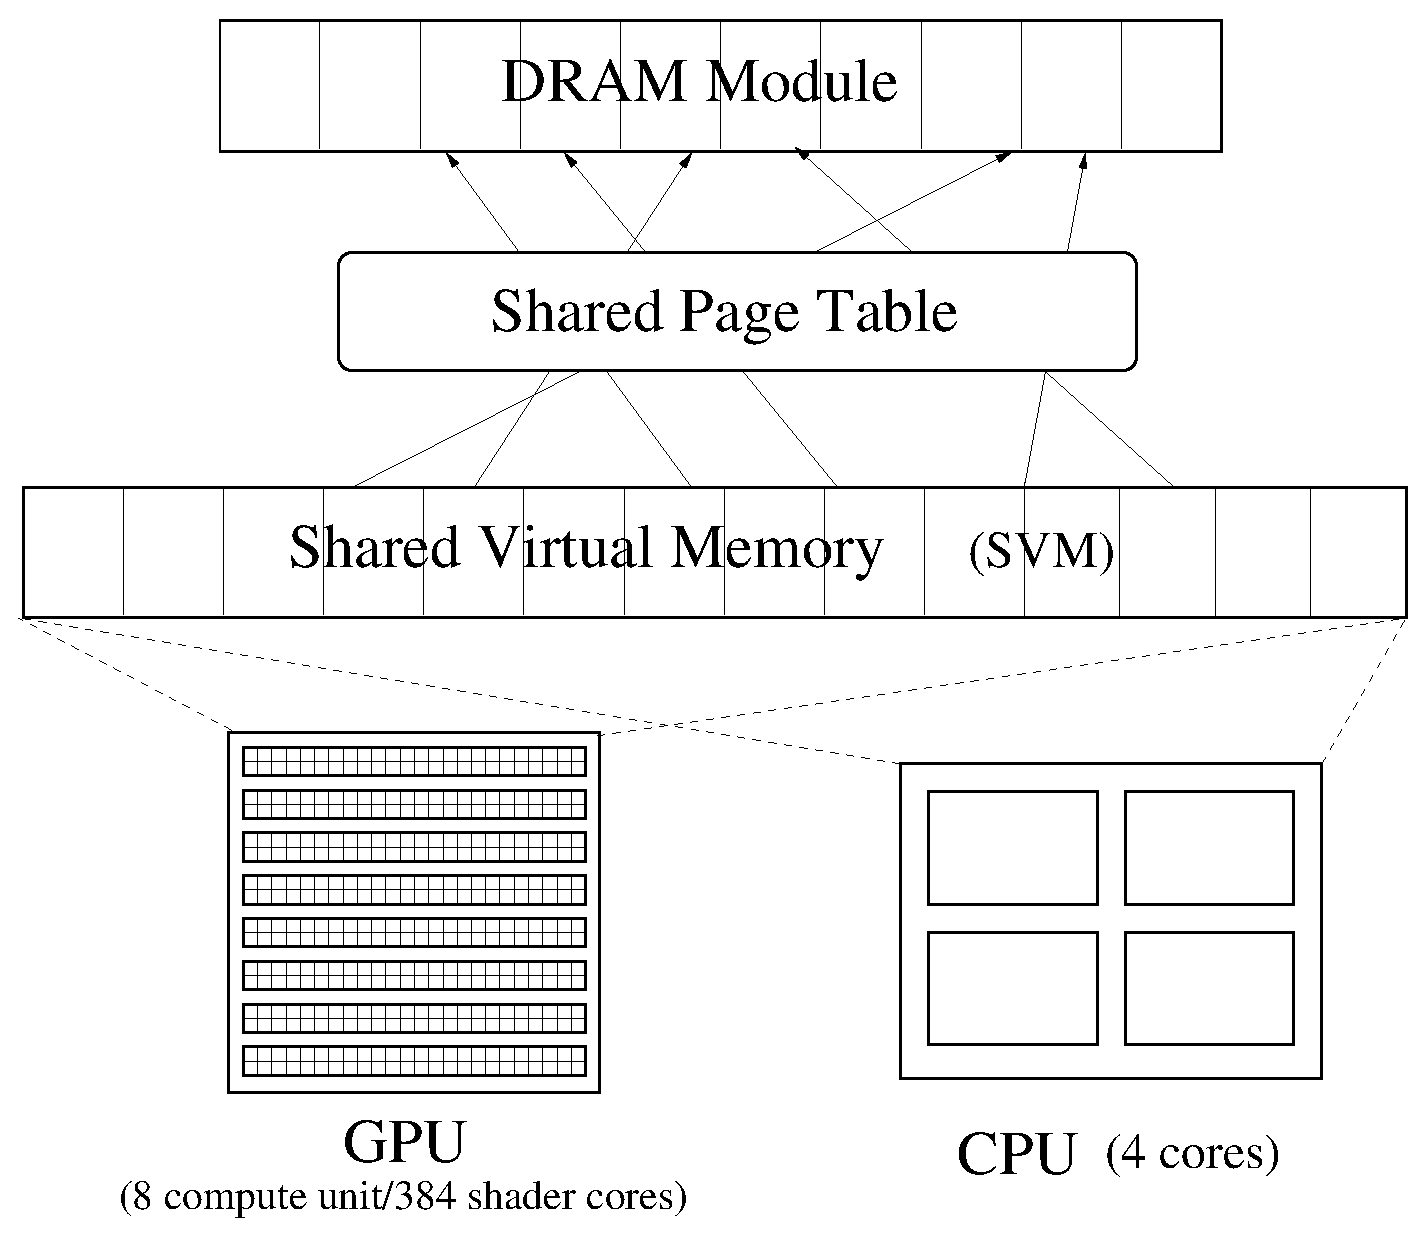
\includegraphics[width=0.8\textwidth]{./figs/carrizo.eps}
            \caption{Carrizo APU with HSA}
            \label{fig:carrizo}
        \end{figure}
        \subsubsection{System Specification}
        The HSA foundation released HSA Platform System Architecture Specification 1.0 \cite{systemspec} in 2015.
        The main purpose of the specification is defining the system requirements which support the HSA programming model and the software infrastructure, from a hardware perspective.
        Figure~\ref{fig:systemspec} illustrates an example of an HSA platform.
        An HSA platform refers to a system involving multiple types of computing devices, 
        which are defined as HSA agents.
        One of the agents needs to be host CPU, and the other usually serve as kernel agents. 
        The host CPU is responsible for running the operating system and setting up \textit{HSA Runtime},
        while kernel agents handle computational tasks from the host CPU by executing HSAIL code.
        HSA requires all HSA agents to be capable of accessing SVM maintained coherently, 
        so data exchange between agents can be accomplished by passing data pointer instead.
        Nevertheless, not all memory regions need to be accessible by all agents (i.e., \textit{Global} segment).
        HSA defines other memory segments (\textit{Group}, \textit{Private}, \textit{Spilled}, etc.), 
        which possess various accessibility by various computing agents or items.
        By manipulating different memory segments, the programmer can utilize data locality in memory hierarchy to improve performance.
        To transmit control signals between agents, HSA specifies \textit{Architected Queuing Language} (AQL) as the protocol. 
        AQL defines several packet types: \textit{agent dispatch}, \textit{kernel dispatch}, \textit{AND barrier} and \textit{OR barrier}, etc.
        An agent pushes tasks wrapped in \textit{kernel dispatch} or \textit{agent dispatch} packets to command queues, 
        and other agents consume the packets, and dispatch the wrapped tasks.
        \textit{AND barrier} and \textit{OR barrier} are pushed to command queues to synchronize execution of agents 
        Another advantage of AQL is allowing \textit{user mode queuing},
        which implies the programmer is allowed to access the command queue via \textit{HSA Runtime API} without OS involving.
        By this mean, the latency from dispatching to execution of a task is thus minimized.
        \vspace{\textfig}
        \begin{figure}[!ht] 
            \centering
            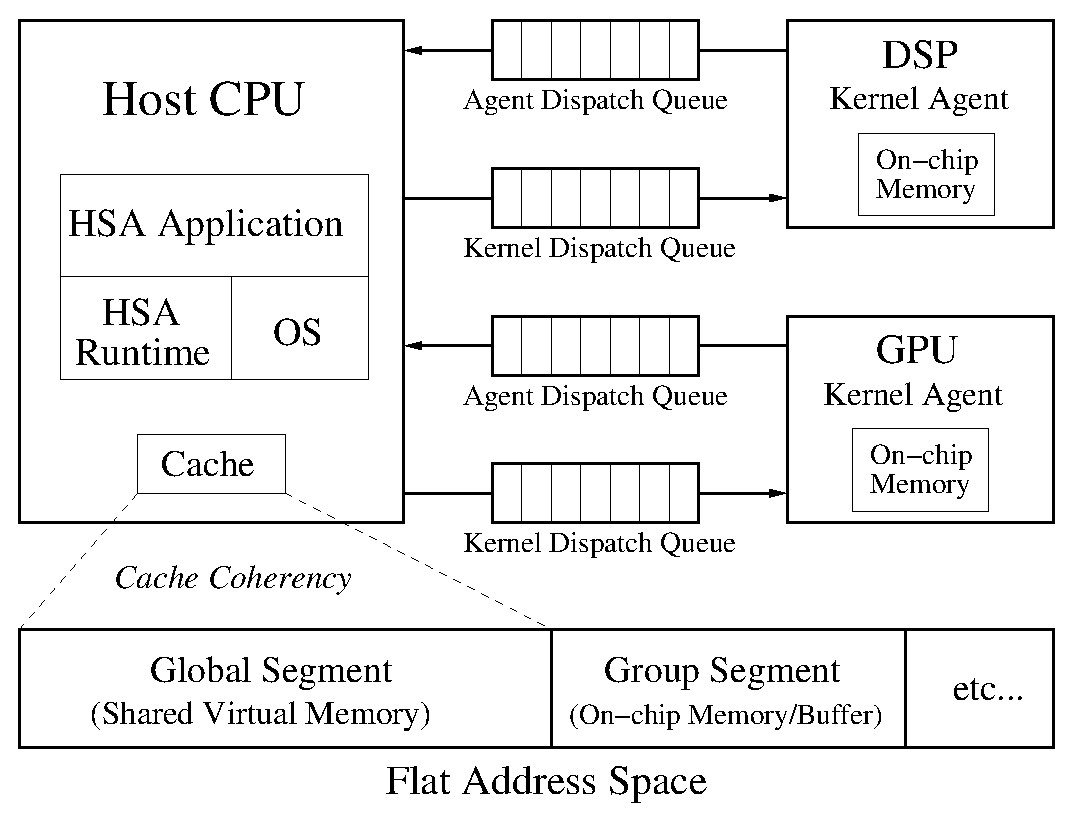
\includegraphics[width=0.85\textwidth]{./figs/systemspec.eps}
            \caption{Example of an HSA Platform}
            \label{fig:systemspec}
        \end{figure}
        \subsubsection{Programming Model}
        To support multiple Instruction Set Architectures (ISAs) for various agents in a single HSA platform,
        HSA foundation drew up /textit{Heterogeneous System Architecture Intermediate Language} (HSAIL)
        With HSAIL, programmers can develop code for HSA in an intermediate form accepted by wide range of agents.
        HSAIL basically adopts the parallel programming model of Single Program Multiple Data (SPMD), 
        which carries out same computation on different data to accelerate applications.
        HSAIL organizes instances of execution in specified hierarchy, which help programmers to manipulate its SPMD model.
        Figure~\ref{fig:grid} presents a graphical view on how HSAIL organizes instances of execution.
        The atomic instance for execution is a work-item, which has dedicated registers and private memory.
        Group of work-items form a work-group, which owns group memory accessed by subordinate work-items only.
        The work-items in a work-group can be arranged in one, two or three dimensional coordinate, 
        and the programmer specifies the number of dimensions as well as the size of each dimension.
        Based on the same principle of arranging instances, all work-groups further form a grid, 
        which provides a global view to all work-items created in an HSAIL program (kernel).
        Work-items within a work-group are executed concurrently in chunks called wavefronts, 
        of which sizes are limited by the number of processing cores (lanes) in the target kernel agent.
        Each work-group and each work-item have work-group ID and work-item ID respectively.
        By manipulating such threading hierarchy, 
        the programmer can control accessibility of data and synchronize the work items in a specific scope without burden.
        \vspace{\textfig}
        \begin{figure}[!ht] 
            \centering
            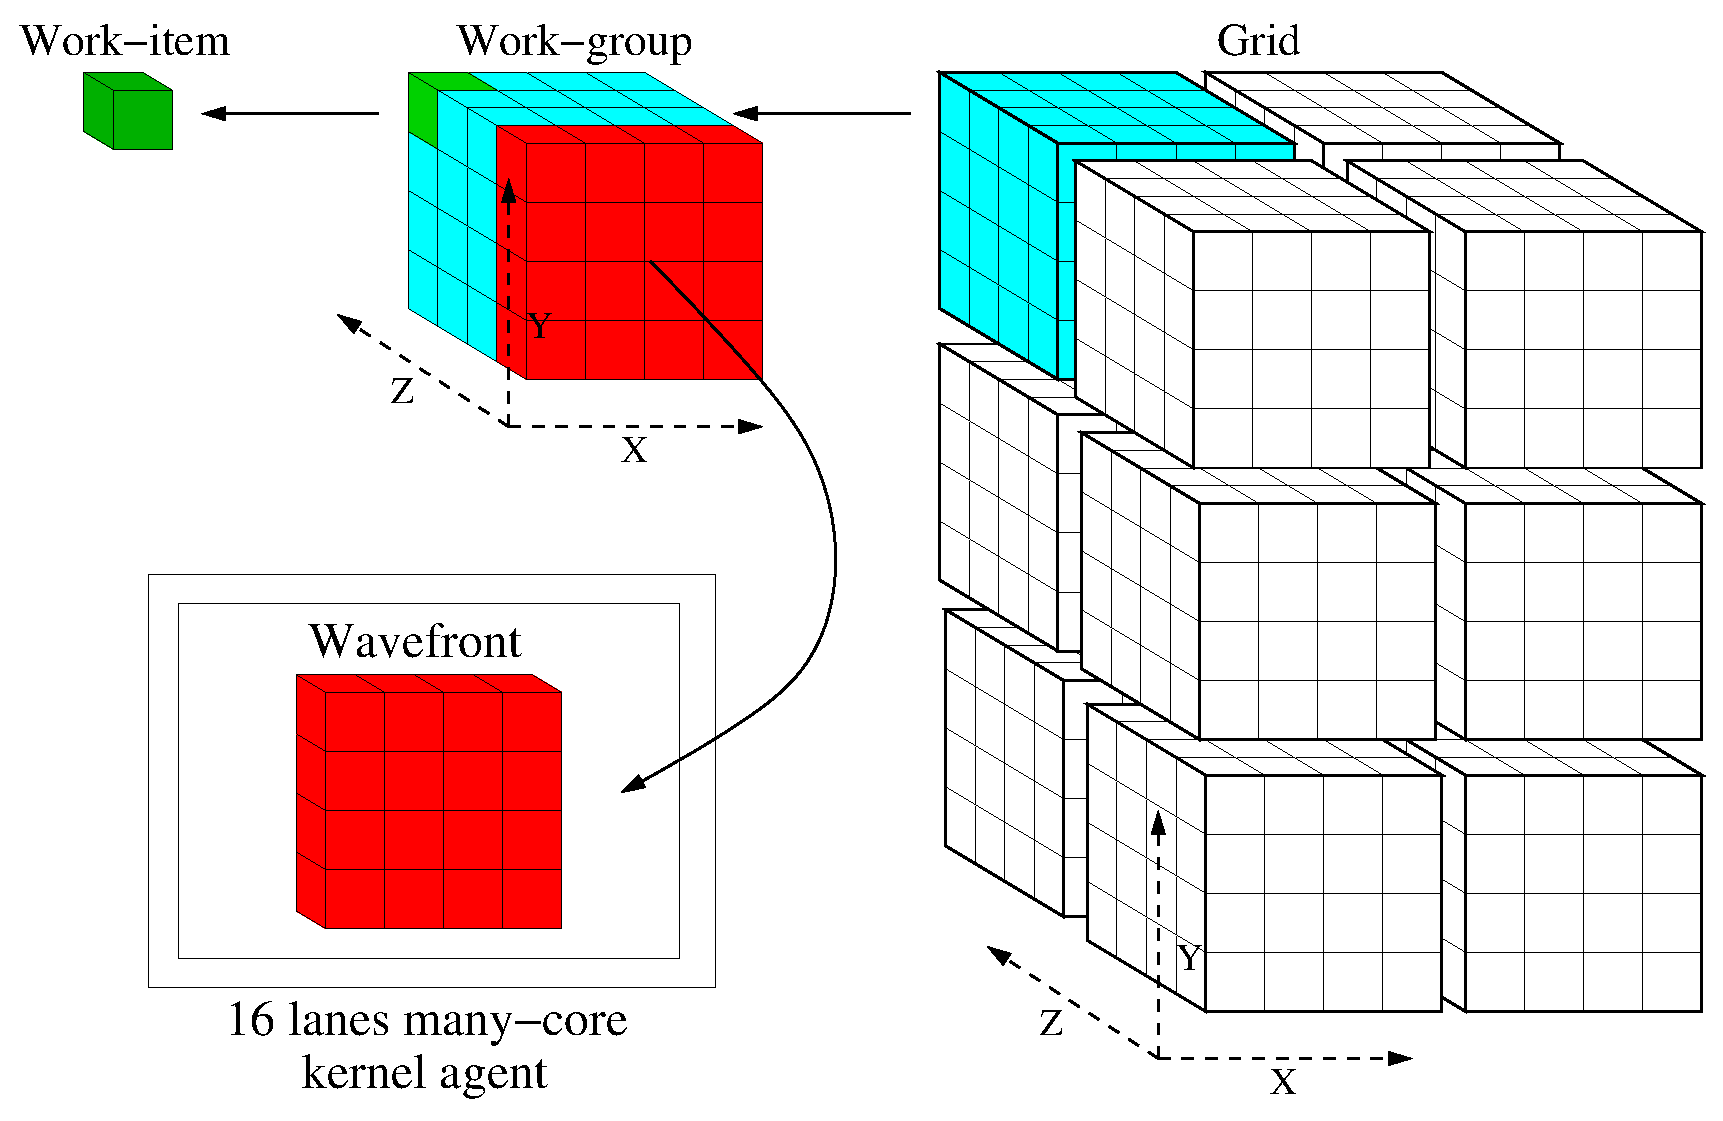
\includegraphics[width=0.85\textwidth]{./figs/grid.eps}
            \caption{Execution hierarchy in HSAIL}
            \label{fig:grid}
        \end{figure}
        % work group, work item warp, memory hierarchy, hqueue, 
        \subsubsection{Software Infrastructure}
        The software infrastructure of HSA is composed of two parts, the compilation tools and the \textit{HSA runtime}.   
        The compilation tools are responsible for generating machine code of specific ISAs from high-level language.
        Figure~\ref{fig:swinf}~(a) illustrates the whole compilation flow of HSA software.
        The programmer develops applications targeting HSA with high-level parallel programming language such as OpenCL, OpenMP or a domain-specific language (DSL).
        The off-line compiler of the hight-level language translate the code to standard HSAIL kernel accepted by all computing devices in an HSA platform.
        Each kind of the computing devices must be recognized by the finalizer, 
        which is composed of several device-specific HSAIL compilers.
        Depending on which device is going to execute the kernel, 
        the finalizer translates the HSAIL to corresponding ISA and completes the code generation flow.
        \\\indent
        On the other hand, the \textit{HSA runtime} bridges HSAIL runtime APIs and agents, as illustrated in Figure~\ref{fig:swinf}~(b).
        With the \textit{HSA runtime}, the programmer is allowed to manipulate system memory and AQL, 
        and thus SVM and \textit{user mode queuing} can be accomplished.
        It is possible that the programmer triggers the finalizer to perform the final stage of compilation at runtime.
        In addition, \textit{HSA runtime} also performs error handling and retrieve system and agent information for users.
        \vspace{\textfig}
        \begin{figure}[!ht] 
            \centering
            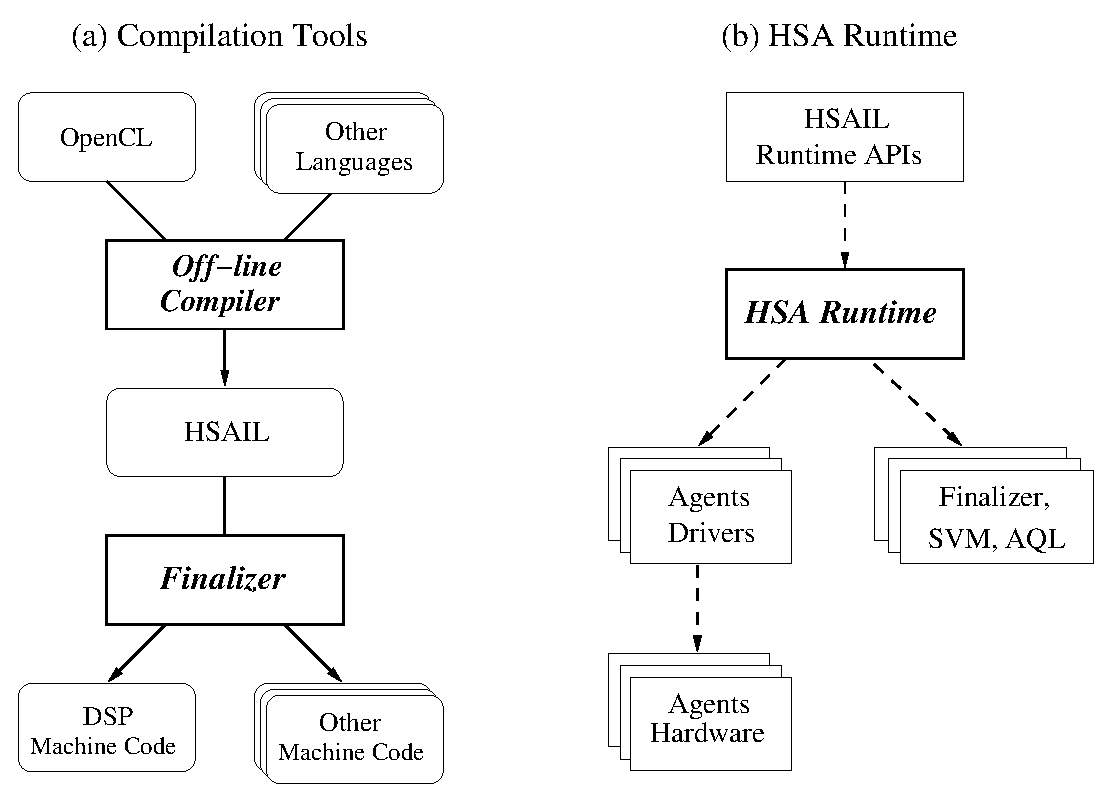
\includegraphics[width=0.85\textwidth]{./figs/swinf.eps}
            \caption{Software Infrastructe of HSA}
            \label{fig:swinf}
        \end{figure}


%
\section{Design and Implementation}
\subsection{DeAr Micro-architecture Design}
Fig.~\ref{fig:micro} illustrates the micro-architecture of DeAr.
Two DeAr threads share the ALU that commonly exist in a RISC datapath.
The demonstrated example includes an adder, a multiplier and a barrel shifter, which are qualified to perform most benchmarks.
The output of each arithmetic unit contains an accumulator latch preserving and forwarding the arithmetic result.
The forwarding mechanism and resolution of structural hazards are both handled by the HDFG-based scheduling.
\\\indent
The RF is physically and symmetrically separated for two threads.
Each thread owns a pair of queue memory as well as a stack memory, 
and these memory modules form the sequential-accessed banked register file (SBRF).
A load-queue and a store-queue serve as the buffer that connects the lower level of the memory hierarchy with the datapath.
They can be accessed from their both sides concurrently in the first-in-first-out (FIFO) fashion.
By preventing queues from empty or full with clever scheduling, the latency of load/store can thus be hidden.
The stack memory, on the other hand, is responsible for the storage of intermediate data.
Any access to the SBRF are simplified to "PUSH" or "POP" instead of conventional random-access.
Such an implicit access mechanism reduces both the code size and decode complexity, 
and constitutes the crucial advantage of DeAr over conventional architectures.
\\\indent
The design of transport triggered data bus (TTDB) was inspired by TTA~\cite{tta}.
TTDB separates the RF from ALU with a set of multiplexers controlled by the instruction unit, 
and forwards data from accumulators to ALU inputs.
It is important to note that, even though the communication among the RF, ALU and accumulators is compacted exhaustively, 
the datapath flexibility is still kept.%
\begin{figure}[t]
    \centering
    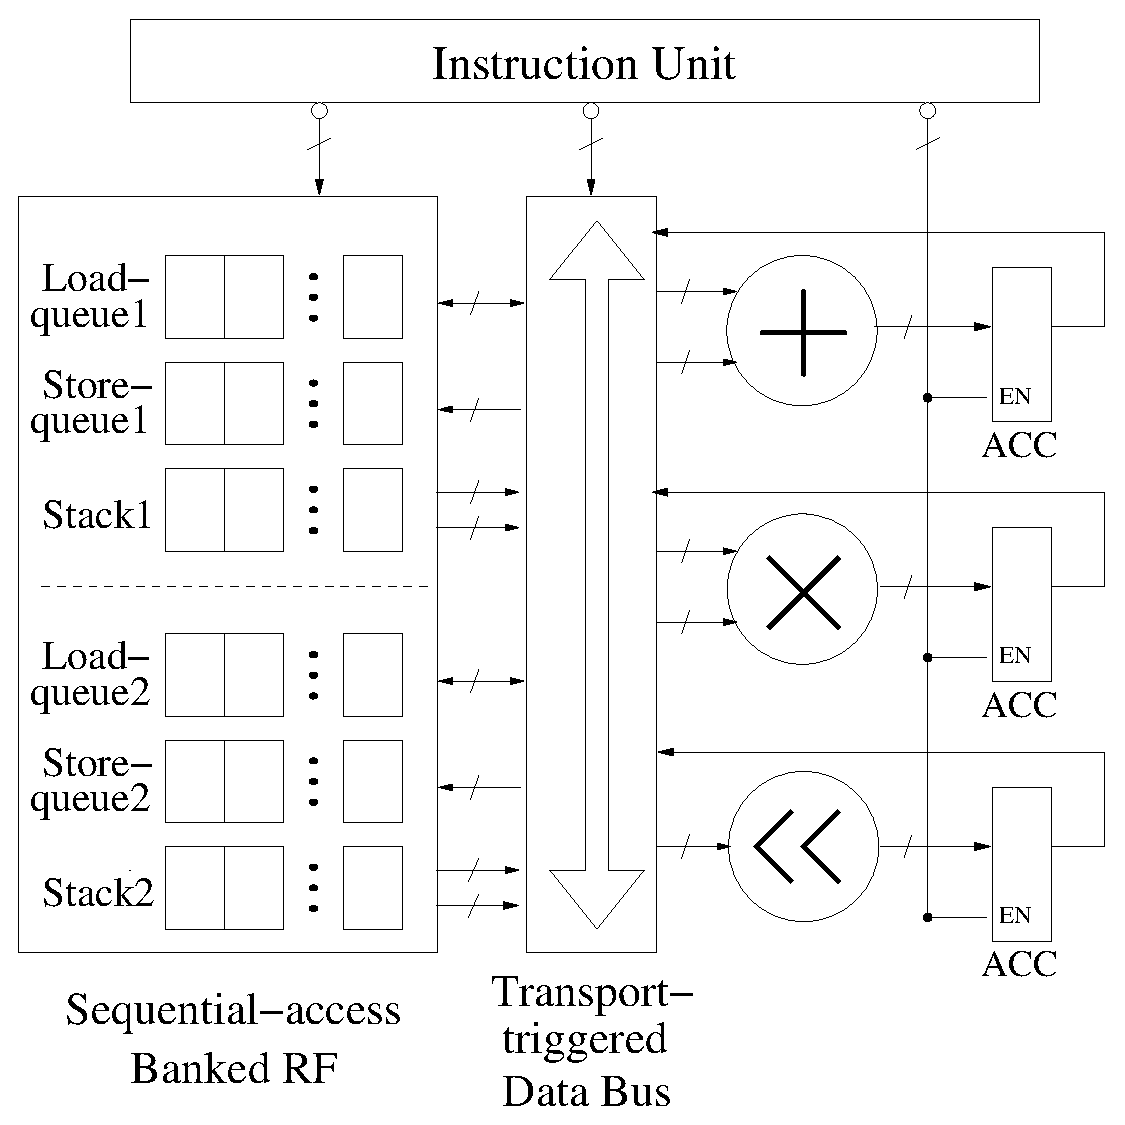
\includegraphics[width=0.33\textwidth]{./figs/micro.eps}
    \caption{Micro-architecture of a DeAr DSP lane}
    \label{fig:micro}
\end{figure}
\subsection{Data Flow Graph to Hierarchical Data Flow Graph}
\label{sec:hdfg}
A data flow graph (DFG), shown in Fig.~\ref{fig:dfg:dfg}, presents dependencies among operations of a program.
We express a DFG with the data structure, $G$, which holds an operation set $V_{op}$ and a dependency set $E_{op}$.
In conventional DSP, scheduling is usually accomplished based on the DFG analysis.
\\\indent
To go beyond DFGs, we propose the hierarchical data flow graph (HDFG).
Fig.~\ref{fig:dfg:hdfg} demonstrates a HDFG, $\bar{G} = (V_{bt}, E_{bt})$, converted from Fig.~\ref{fig:dfg:dfg}.
Properties of HDFGs include: 
\textbf{(1)} Cascaded operations ($op$) form a super node ($sn$), and an isolated $op$ forms a $sn$ directly. 
Within a $sn$, an $op$ forwards data to the next one.
\textbf{(2)} Neighboring $sn$s form a full binary tree ($bt$), and isolated $sn$ forms a $bt$ directly.
These $bt$s further form a set of vertices, $V_{bt}$.
Within a $bt$, a parent $sn$ receives the first operand popped from the stack and the second one forwarded via TTDB.
\textbf{(3)} Dependencies among $op$s that cross $bt$s are inherited by the $bt$s they belong to.
These inherited dependencies form a set of edges, $E_{bt}$, of $V_{bt}$.
\textbf{(4)} A $bt$ without any in-edge existing in $\bar{G}$ (i.e., $bt \in V_{bt}\ |\ \textrm{deg}^-(bt) = 0$) is free to be scheduled. 
After scheduled, the $bt$ and its edges are erased from the $\bar{G}$.%
\setlength{\textfloatsep}{10pt}% Remove \textfloatsep
\begin{figure}[t]
\begin{center}
\subfigure[DFG example]
{
\label{fig:dfg:dfg}
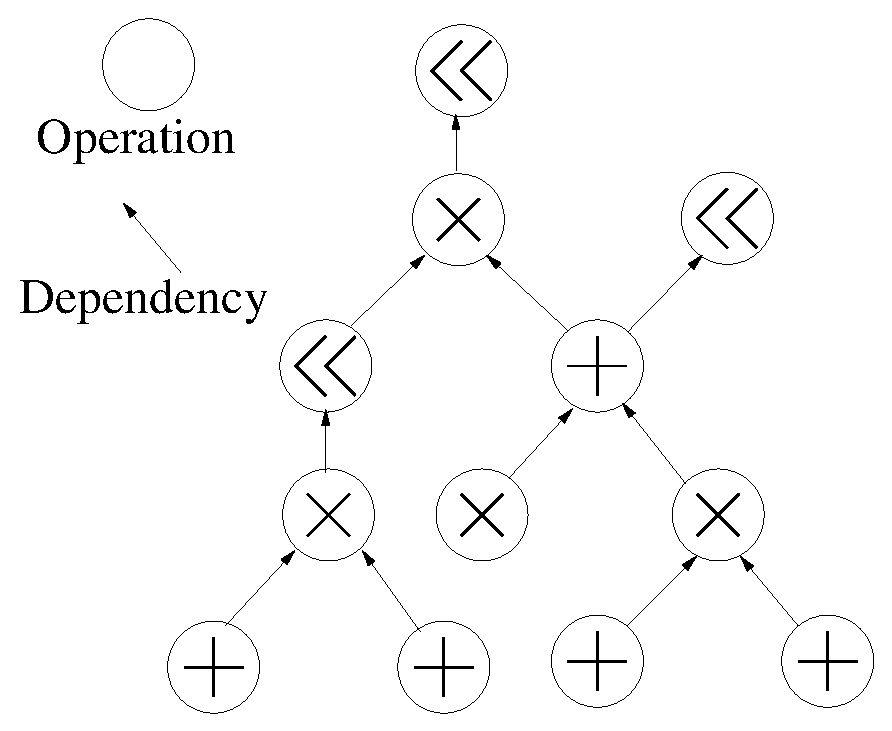
\includegraphics[width=0.19\textwidth]{figs/dfg.eps}
}%
\hspace{0.5em}
\subfigure[Corresponding HDFG]
{
\label{fig:dfg:hdfg}
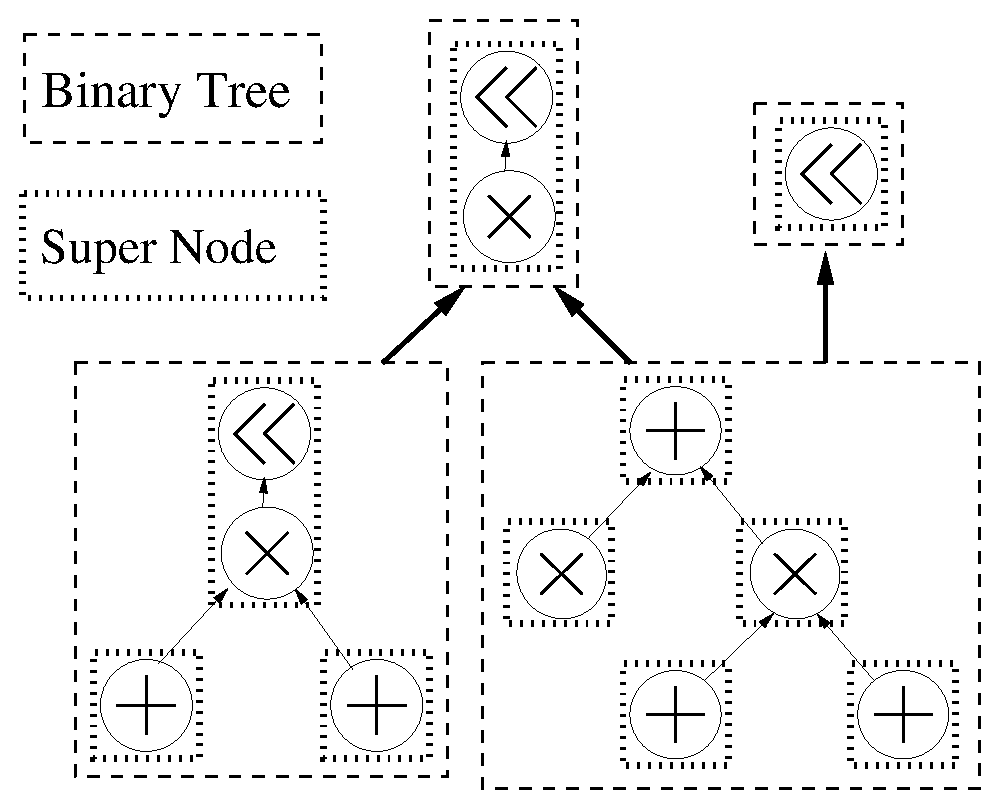
\includegraphics[width=0.21\textwidth]{figs/hdfg.eps}
}
\end{center}
\caption{Conversion from DFG to HDFG}
\label{fig:dfg}
\end{figure}
\subsection{HDFG-based Scheduling}
\label{sec:scheduling}
The goal of the DeAr scheduler is generating the binary code with maximum ILP, maximum data forwarding rate, 
and minimum stack memory consumption of each thread.
To achieve the goal, we present a novel scheduling algorithm, 
\textproc{HDFG-based scheduling}, which is shown in Algorithm~\ref{alg}.
The algorithm takes an HDFG ($\bar{G}$) as the input and generates the output binary code ($X_{final}$).
\\\indent
The scheduler firstly completes the \textit{Inter-tree scheduling phase}
for the purpose of dispatching operations from independent $bt$s to two threads.
Line~\ref{line:interws}--\ref{line:interwe}, enclosed by a while loop, is the \textit{Inter-tree scheduling phase}, 
where the scheduler performs symmetric steps for two threads.
If there is a thread with an empty operation-list, 
the scheduler searches $\bar{G}$ and selects a free $bt$ randomly, 
and assigns operations in the $bt$ sorted by higher-subtree-first postorder-traversal (\textproc{HFPT Sort}) to its operation-list.
The postorder-traversal ensures that children are listed in front of their parent, 
and the higher-subtree-first policy ensures that nodes of the higher subtree are listed in front of ones of its sibling, 
which minimizes the stack memory consumption.
Next, it performs \textproc{ALU Allocation} for two operation-lists.
This subroutine dispatches operations allowed to execute concurrently, 
and generates the code segment containing the dispatched operations and control signal for SBRF and TTDB.
It applies Dynamic Programming (DP)~\cite{dp} to determine which thread should stall when the ALU conflict occurs.
After \textproc{ALU Allocation}, at least one operation-list is consumed, 
and the returned code segment is accumulated with the current segment.
As shown in Line~\ref{line:intercon}, we use $\oplus$ to denote the code accumulation.
The loop proceeds until all $bt$s in $\bar{G}$ are scheduled.
\\\indent
Nevertheless, it is very likely that one of operation-lists has operations remaining at the last iteration.
Line~\ref{line:interis}--\ref{line:interie} illustrate such a scenario.
Remaining operations are thus reverted to the original form of $bt$ by the subroutine \textproc{Restore Subtree from list},
and a remaining subtree, $bt_{remain}$, is obtained.%
\\\indent
To deal with the $bt_{remain}$, 
the scheduler performs the \textit{Intra-tree scheduling phase}, 
which dispatches operations from two subtrees of the $bt_{remain}$ to two threads respectively.
Line~\ref{line:intra:ws}--\ref{line:intra:we} show a while loop for \textit{Intra-tree scheduling phase}.
A crucial strategy applied here is, partitioning $bt_{remain}$ into three parts:
the root node, left and right subtrees.
Since operations in the root must be handled sequentially, 
we can dispatch them directly with a single thread (thread 1), 
and obtain a binary code segment, $X_{single}$.
Then, by treating the left and right subtrees as independent trees, 
we can perform similar steps applied in the \textit{Inter-tree scheduling phase}.
We manipulate \textproc{HFPT Sort} and \textproc{ALU Allocation} again, and obtain another binary code segment, $X_{intra}$.
By repeating above steps, $bt_{remain}$ keeps shrinking while $X_{intra}$ and $X_{single}$ keep accumulating,
until all operations left in $bt_{remain}$ are dispatched.
Finally, we concatenate $X_{inter}$, $X_{intra}$ and $X_{single}$,
and obtain the complete code $X_{final}$.
%-----------Inter-tree-------------
%\setlength{\textfloatsep}{0pt}% Remove \textfloatsep
\begin{algorithm}[t]
{
        \fontsize{8pt}{9pt}\selectfont
    \caption{\textproc{HDFG-based Scheduling}}
    \begin{algorithmic}[1]
        \Require    HDFG $\bar{G} = (V_{bt}, E_{bt})$
        \Ensure     $X_{final}$
        \State $X_{inter},X_{intra},X_{single}\Leftarrow NULL$       %\Comment{Initialize $X_{inter}$}
        \While{$V_{bt} \neq \emptyset$} \label{line:interws}
        \Comment \textit{Inter-tree scheduling phase}
        \If{$op\_list_{thread1} = \emptyset$}
        %\State Select $bt \ni \sum_{bt \in V_{bt}}\textrm{deg}^-(bt) = 0$
        \State $op\_list_{thread1} \Leftarrow$ \Call{HFPT Sort }{$bt$}, where $bt\in V_{bt}\ |\ \textrm{deg}^-(bt) = 0$ 
        %\State Erase $bt$ and its edges from $\bar{G}$
        \EndIf
        \If{$op\_list_{thread2} = \emptyset$}
        \State $op\_list_{thread2} \Leftarrow$ \Call{HFPT Sort }{$bt$}, where $bt\in V_{bt}\ |\ \textrm{deg}^-(bt) = 0$
        %\State Erase $bt$ and its edges from $\bar{G}$
        \EndIf
        \State $X_{1} \Leftarrow X_{1}\oplus$\Call{ALU Alloc}{$op\_list_{thread1}$,$op\_list_{thread2}$} \label{line:intercon}
        \EndWhile \label{line:interwe}
        \If{$work\_queue_{thread1} \neq \emptyset$} \label{line:interis}
        \State $bt_{remain} \Leftarrow$ \Call{Restore-Subtree}{$op\_list_{thread1}$}
        \State Clear $work\_queue_{thread1}$
        \ElsIf{$work\_queue_{thread2} \neq \emptyset$}
        \State $bt_{remain} \Leftarrow$ \Call{Restore-Subtree}{$op\_list_{thread2}$}
        \State Clear $work\_queue_{thread2}$
        \Else
        \State $bt_{remain} \Leftarrow NULL$
        \EndIf \label{line:interie}
        \While{$bt_{remain} \neq \emptyset$}    \label{line:intra:ws}
        \Comment \textit{Intra-tree scheduling phase}
        \State $X_{single} \Leftarrow$ \Call{Gen Code Single Thread }{$bt_{root}$} $\oplus X_{single}$
        \State $op\_list_{thread1} \Leftarrow$ \Call{HFPT Sort }{$bt_{left-subtree}$}
        \State $op\_list_{thread2} \Leftarrow$ \Call{HFPT Sort }{$bt_{right-subtree}$}
        \State $X_{body} \Leftarrow X_{body} \oplus$ \Call{ALU Alloc }{$op\_list_{thread1}$, $op\_list_{thread2}$}
        \If{$work\_queue_{thread1} \neq \emptyset$}
        \State $bt_{remain} \Leftarrow$ \Call{Restore Subtree}{$work\_queue_{thread1}$}
        \State Clear $work\_queue_{thread1}$
        \ElsIf{$work\_queue_{thread2} \neq \emptyset$}
        \State $bt_{remain} \Leftarrow$ \Call{Restore Subtree}{$work\_queue_{thread2}$}
        \State Clear $work\_queue_{thread2}$
        \Else
        \State $bt_{remain} \Leftarrow NULL$
        \EndIf
        \EndWhile   \label{line:intra:we}
        \State $X_{final} \Leftarrow X_{inter} \oplus X_{intra} \oplus X_{single}$
        \State \Return{$X_{final}$}
    \end{algorithmic}%
    \label{alg}
}
\end{algorithm}



\section{Performance Evaluation}
\subsection{Experiment Setup}
\label{sec:evaluation:setup}
%In this chapter, we present the performance evaluation of DeAr and demonstrate its capability of efficient arithmetic.
Two benchmark suites were prepared for the experiment.
The first one is adapted from the BLAS~\cite{blas} library, 
which contains various matrix arithmetic subprograms that are crucial in wireless communication.
The second one includes general DSP kernels (GDSPK) selected from classic DSP benchmark suites, BDTI~\cite{bdti} and DSPstone~\cite{dspstone}.
Table.~\ref{tab:op} lists the operation profiling of two benchmark suites, 
where each subprogram/kernel comprises three primitive operations, addition, multiplication and shifting.
\setlength{\textfloatsep}{0pt}
\begin{table}[h]%
\centering%
\caption{Operation profiling of two benchmark suites}%
\label{tab:op}%
\resizebox{\columnwidth}{!}%
{%
\begin{tabular}{|c|c|c|c|c|c|c|c|c|}%
\hline%
\multicolumn{9}{|c|}{\textbf{Basic linear algebra subprograms (BLAS)}} \\ \hline%
Benchmark              & AXPY   & MV     & MM      & INV      & CAXPY  & CMV  & CMM    & CINV  \\ \hline
\# add            &  32    &  56    &   48    &    75    &  128   & 132  &   90   &  88   \\ \hline
\# mul            &  32    &  64    &   64    &   172    &  128   & 144  &  108   & 114   \\ \hline
\# sht            &   0    &   0    &    0    &     0    &    0   &   0  &    0   &   0   \\ \hline
\# op             &  64    & 120    &  112    &   247    &  256   & 276  &  198   & 202   \\ \hline
\multicolumn{9}{|c|}{\textbf{General DSP kernels (GDSPK)}}                     \\ \hline
Benchmark              & FIR    & CFIR   & LPFIR   & Biquad   & IT     & DCT  & IMDCT  & FFT   \\ \hline
\# add            & 15     &  62    &   15    &    8     &  32    &  29  &   21   &  23   \\ \hline
\# mul            & 16     &  64    &    8    &    9     &   0    &  12  &   11   &  10   \\ \hline
\# sht            &  0     &   0    &    0    &    0     &  10    &   9  &    9   &   0   \\ \hline
\# op             & 31     & 126    &   23    &   17     &  42    &  50  &   41   &  33   \\ \hline
\end{tabular}%
}%
\end{table}%
Various architectures, DeAr, scalar, VLIW, and composite-ALU \cite{cascade} were evaluated for comparison. 
Note that \cite{cascade} is a class of ASIP, and we evaluated it with two ALU configurations, M-S-A and A-M-S.
\subsection{Pre-synthesis Analysis}
    Under a certain throughput requirement, operations per cycle (OPC) determines the timing constraint for hardware synthesis, 
    where higher OPC brings looser timing constraint, which results in lower cost from the post-synthesis hardware.
    Table.~\ref{tab:opc} profiles the OPC of various DSPs with the assumption that every operation consumes exactly one clock cycle.
    The OPC of the scalar processor is fixed to 1.0 because of the limitation of the single-issue datapath.
    On the contrary, benefiting from the wide issue-width and large port number of RF, VLIW gains the best OPC in all benchmarks.
    The OPC of DeAr is limited by the access pattern to the RF which either be LIFO or FIFO, 
    and thus it is not possible for DeAr to outperform the VLIW in regard to OPC.
    Nevertheless, by leveraging the HDFG-based scheduling,
    DeAr still gains approximate OPC of the VLIW, with only 1.11\% and 4.26\% loss in two benchmark suites.
    On the other hand, the OPC of composite-ALU is highly correlated with the benchmark characteristic. 
    On average, the MSA order gains better OPC than the AMS order, 
    but the former still underperforms 3-way VLIW by 12.3\% and 17.7\% in the benchmarks suites.%
\setlength{\textfloatsep}{0pt}%
\begin{table}[h]%
\centering%
\caption{Operations per cycle profiling}%
\label{tab:opc}%
\resizebox{\columnwidth}{!}%
{%
\begin{tabular}{|c|c|c|c|c|c|c|c|c|c|}%
\hline
\multicolumn{10}{|c|}{\textbf{Basic linear algebra subprograms (BLAS)}} \\ \hline
Benchmark  &  AXPY  &  MV  &  MM  &  MINV  &  CAXPY  &  CMV  &  CMM  &  CMINV  &  Average \\ \hline 
VLIW  &   1.94  &   1.85  &   1.72  &   1.44  &   1.97  &   1.89  &   1.80  &   1.76  &   1.79     \\ \hline 
DeAr  &   1.94  &   1.85  &   1.72  &   1.40  &   1.97  &   1.89  &   1.80  &   1.62  &   1.77     \\ \hline
Comp.-MSA  &   2.00  &   1.88  &   1.75  &   1.37  &   1.33  &   1.35  &   1.38  &   1.53  &   1.57     \\ \hline 
Comp.-AMS  &   1.00  &   1.00  &   1.00  &   1.02  &   1.00  &   1.00  &   1.00  &   1.04  &   1.01     \\ \hline 
Scalar  & 1.0  & 1.0  & 1.0  & 1.0  & 1.0  & 1.0  & 1.0  & 1.0  & 1.0 \\ \hline 
\multicolumn{10}{|c|}{\textbf{General DSP application kernels (GDSPK)}}                     \\ \hline
Benchmark  &  FIR  &  CFIR  &  LPFIR  &  Biquad  &  IT  &  DCT  &  IMDCT  &  FFT  &  Average \\ \hline 
        VLIW  &   1.82  &   1.91  &   1.67  &   1.55  &   1.33  &   1.61  &   1.86  &   1.38  &   1.64     \\ \hline 
        DeAr  &   1.82  &   1.91  &   1.67  &   1.55  &   1.33  &   1.47  &   1.46  &   1.32  &   1.57     \\ \hline 
        Comp.-MSA  &   1.94  &   1.34  &   1.44  &   1.42  &   1.31  &   1.14  &   1.28  &   1.06  &   1.35     \\ \hline 
        Comp.-AMS  &   1.00  &   1.00  &   1.53  &   1.21  &   1.14  &   1.61  &   1.52  &   1.27  &   1.29     \\ \hline 
        Scalar  & 1.0  & 1.0  & 1.0  & 1.0  & 1.0  & 1.0  & 1.0  & 1.0  & 1.0 \\ \hline 
    \end{tabular}%
}%
\end{table}%
\subsection{Synthesis Result and Analysis}
In this part, we present hardware synthesis results with the throughput requirement varying from 50 to 1000 MOPS, 
We implemented aforementioned designs with UMC 65nm cell library, 
and measured their area and power dissipation with Synopsys Design Compiler and Synopsys Prime Time under the timing constraint based on the average of Table.~\ref{tab:opc}.
Synthesis failures owing to timing violation reported by the tool would remain corresponding entries empty in figures.
%\subsubsection{Area}
\\\indent 
Figure~\ref{chart:area} shows the area improvement of DeAr over with other architectures.
DeAr saves 24.5\%--21.1\% of area against VLIW.
The area of the VLIW architecture is dominated by RF, 
which demands complicated interconnection among ports and registers to facilitate centralized organization.
By contrast, DeAr, which trades off the connectivity by adopting the banked RF, can thus achieve significant area improvement.
Since RF access is not the crucial issue affecting the critical path for both VLIW and DeAr, 
the correlation between throughput and save percentage is inconspicuous.
\\\indent On the other hand, DeAr achieves 21.2\%--5.6\% area improvement against composite-ALU with the MSA order.
When compared with the AMS order, the save percentage becomes 17.2\%--5.3\%.
Composite-ALU architectures reduce area by using fewer ports on the RF.
Nevertheless, the area burden caused by the centralized RF still exists.
Another drawback of composite-ALU architectures is long critical path in the ALU, 
which leads to sharp area growth as throughput increasing.
\\\indent Benefiting from the simple datapath, 
the scalar costs lowest area when throughput was low.
However, the low OPC of scalar becomes the terrible burden on achieving high throughput.
The area of scalar exceeds the one of DeAr while throughput is above 600 MOPS.
Consequently, DeAr achieves lowest area among five designs while throughput is high.%
\\\indent
The power dissipation in CMOS devices consists of dynamic power and static power.
In our experiment, the former is the dominating factor, which accounts for 98\%--70\% of the total dissipation, 
owing to the cell library characteristic, 
As a result, our analysis focuses on the dynamic power, 
which is proportional to the product of clock rate $f$, logic switching rate $\alpha$ and the load $C_L$ of each cell.
\\\indent
Figure~\ref{chart:power} shows the power dissipation improvement of DeAr compared with other architectures.
DeAr saves 22.7\%--15.1\% against VLIW.
%and 21.1\%--16.5\% (BLAS) and 17.3\%--13.1\% (GDSPK) of power compared with the 3-way VLIW.
The power improvement achieved by DeAr is attributed to the low RF access rate achieved by the HDFG-based scheduling, which reduces $\alpha$, 
and the banked RF organization, which reduces $C_L$.
\\\indent
The power dissipation of composite-ALU is significantly influenced by its ALU order.
Below 600 MOPS, DeAr achieves 46.9\%--41.2\% power reduction against AMS, 
but only achieves 7.1\%--2.6\% against MSA.  
Compared with AMS, MSA benefits from high OPC, which reduces $f$, and low RF access rate, which reduces $\alpha$, 
so it stays competitive against DeAr in regard to power dissipation.
However, the sharp area growth of composite-ALU also drives severe growth of $C_L$.
As a result, the power dissipation of MSA gradually diverges from the one of DeAr as throughput increasing, 
and DeAr achieves 22.5\%--8.7\% power improvement against MSA while throughput is above or equal to 600 MOPS.
\\\indent
Although the scalar processor cost low area, which implies low $C_L$, 
the worst OPC and RF access rate among designs brings unfavorable $f$ and $\alpha$, 
which result in severe power dissipation. 
Compared with the scalar, DeAr saves 52.1\%--45.8\% of power while below 700 MOPS, 
and the synthesis for scalar fails while above 700 MOPS.
In regard to power dissipation, DeAr achieves the best result among designs regardless throughput.%
\setlength{\textfloatsep}{10pt}% Remove \textfloatsep
\begin{figure}
\begin{center}
\subfigure[b][Area improvement]
{
\label{chart:area}
\includegraphics[width=0.25\textwidth]{charts/area_average_save.eps}%
}%
\subfigure[b][Power dissipation improvement]
{
\label{chart:power}
\includegraphics[width=0.25\textwidth]{charts/power_average_save.eps}
}
\end{center}
\caption{Performance improvement of DeAr}
\label{chart:area}
\end{figure}


\section{Conclusions and Future Work}
In this work, we propose a high throughput, power-efficient and flexible DSP design, DeAr,
which is suitable for fast-evolving wireless communication protocols.
DeAr manipulates SMT in the datapath to improve the hardware utilization, 
and its compact design reduces the cost of power and area.
It also features implicit RF access to improve the code density.
By leveraging the proposed HDFG-based scheduling, 
DeAr exhaustively forwards data for ALU, 
and has only 1.11\% (BLAS) and 4.26\% (GDSPK) loss in OPC against VLIW in spite of its hardware simplification,
With identical ALU, RF resources and the throughput requirement ranging from 50 to 1000 MOPS, DeAr improves 20.3\% to 13.1\% and 31.8\% 2.2\% of power, 36.1\% to 31.5\% and 28.2\% to 5.7\% of area, compared with VLIW and composite-ALU (an ASIP implementation) respectively.
\\\indent
Our future work will focus on scaling up DeAr to the many-core architecture facilitating data-intensive computation.
The scheduling approach in this work is not suitable for massive threads management, 
which is usually performed dynamically by a dedicated hardware (i.e., warp scheduler in GPU).
Applying such a thread management unit to DeAr while keeping the hardware simplicity requires more studies.








% An example of a floating figure using the graphicx package.
% Note that \label must occur AFTER (or within) \caption.
% For figures, \caption should occur after the \includegraphics.
% Note that IEEEtran v1.7 and later has special internal code that
% is designed to preserve the operation of \label within \caption
% even when the captionsoff option is in effect. However, because
% of issues like this, it may be the safest practice to put all your
% \label just after \caption rather than within \caption{}.
%
% Reminder: the "draftcls" or "draftclsnofoot", not "draft", class
% option should be used if it is desired that the figures are to be
% displayed while in draft mode.
%
%\begin{figure}[!t]
%\centering
%\includegraphics[width=2.5in]{myfigure}
% where an .eps filename suffix will be assumed under latex, 
% and a .pdf suffix will be assumed for pdflatex; or what has been declared
% via \DeclareGraphicsExtensions.
%\caption{Simulation results for the network.}
%\label{fig_sim}
%\end{figure}

% Note that the IEEE typically puts floats only at the top, even when this
% results in a large percentage of a column being occupied by floats.


% An example of a double column floating figure using two subfigures.
% (The subfig.sty package must be loaded for this to work.)
% The subfigure \label commands are set within each subfloat command,
% and the \label for the overall figure must come after \caption.
% \hfil is used as a separator to get equal spacing.
% Watch out that the combined width of all the subfigures on a 
% line do not exceed the text width or a line break will occur.
%
%\begin{figure*}[!t]
%\centering
%\subfloat[Case I]{\includegraphics[width=2.5in]{box}%
%\label{fig_first_case}}
%\hfil
%\subfloat[Case II]{\includegraphics[width=2.5in]{box}%
%\label{fig_second_case}}
%\caption{Simulation results for the network.}
%\label{fig_sim}
%\end{figure*}
%
% Note that often IEEE papers with subfigures do not employ subfigure
% captions (using the optional argument to \subfloat[]), but instead will
% reference/describe all of them (a), (b), etc., within the main caption.
% Be aware that for subfig.sty to generate the (a), (b), etc., subfigure
% labels, the optional argument to \subfloat must be present. If a
% subcaption is not desired, just leave its contents blank,
% e.g., \subfloat[].


% An example of a floating table. Note that, for IEEE style tables, the
% \caption command should come BEFORE the table and, given that table
% captions serve much like titles, are usually capitalized except for words
% such as a, an, and, as, at, but, by, for, in, nor, of, on, or, the, to
% and up, which are usually not capitalized unless they are the first or
% last word of the caption. Table text will default to \footnotesize as
% the IEEE normally uses this smaller font for tables.
% The \label must come after \caption as always.
%
%\begin{table}[!t]
%% increase table row spacing, adjust to taste
%\renewcommand{\arraystretch}{1.3}
% if using array.sty, it might be a good idea to tweak the value of
% \extrarowheight as needed to properly center the text within the cells
%\caption{An Example of a Table}
%\label{table_example}
%\centering
%% Some packages, such as MDW tools, offer better commands for making tables
%% than the plain LaTeX2e tabular which is used here.
%\begin{tabular}{|c||c|}
%\hline
%One & Two\\
%\hline
%Three & Four\\
%\hline
%\end{tabular}
%\end{table}


% Note that the IEEE does not put floats in the very first column
% - or typically anywhere on the first page for that matter. Also,
% in-text middle ("here") positioning is typically not used, but it
% is allowed and encouraged for Computer Society conferences (but
% not Computer Society journals). Most IEEE journals/conferences use
% top floats exclusively. 
% Note that, LaTeX2e, unlike IEEE journals/conferences, places
% footnotes above bottom floats. This can be corrected via the
% \fnbelowfloat command of the stfloats package.





% trigger a \newpage just before the given reference
% number - used to balance the columns on the last page
% adjust value as needed - may need to be readjusted if
% the document is modified later
%\IEEEtriggeratref{8}
% The "triggered" command can be changed if desired:
%\IEEEtriggercmd{\enlargethispage{-5in}}

% references section

% can use a bibliography generated by BibTeX as a .bbl file
% BibTeX documentation can be easily obtained at:
% http://mirror.ctan.org/biblio/bibtex/contrib/doc/
% The IEEEtran BibTeX style support page is at:
% http://www.michaelshell.org/tex/ieeetran/bibtex/
%\bibliographystyle{IEEEtran}
% argument is your BibTeX string definitions and bibliography database(s)
%\bibliography{IEEEabrv,../bib/paper}
%
% <OR> manually copy in the resultant .bbl file
% set second argument of \begin to the number of references
% (used to reserve space for the reference number labels box)

\bibliographystyle{IEEEtran}
\bibliography{apccas}



% that's all folks
\end{document}


